

\mode<presentation>
{
  \usetheme{boxes}
  %\useoutertheme{infolines}
  % með efnisyfirliti: Szeged, Frankfurt 
  % án efnisyfirlits: Pittsburgh
  % áhugavert: CambridgeUS, Boadilla
  %\setbeamercovered{transparent} %gegnsætt
  \setbeamercovered{invisible}

\defbeamertemplate*{footline}{infolines theme}
{
  \leavevmode%
  \hbox{%
  \begin{beamercolorbox}[wd=.333333\paperwidth,ht=2.25ex,dp=1ex,center]{author in head/foot}%
  %  \usebeamerfont{author in head/foot}\insertshortauthor~~\beamer@ifempty{\insertshortinstitute}{}{(\insertshortinstitute)}
  \end{beamercolorbox}%
  \begin{beamercolorbox}[wd=.333333\paperwidth,ht=2.25ex,dp=1ex,center]{title in head/foot}%
   % \usebeamerfont{title in head/foot}\insertshorttitle
  \end{beamercolorbox}%
  \begin{beamercolorbox}[wd=.333333\paperwidth,ht=2.25ex,dp=1ex,right]{date in head/foot}%
    %\usebeamerfont{date in head/foot}\insertshortdate{}\hspace*{2em}
    \insertshortlecture.\insertframenumber{} / \insertshortlecture.\inserttotalframenumber\hspace*{2ex} 
  \end{beamercolorbox}}%
  \vskip0pt%
}
\resetcounteronoverlays{rtaskno} %Does not increase counter rtaskno on \pause in beamer


}


\usepackage[english,icelandic]{babel}
\usepackage[utf8]{inputenc}
\usepackage{t1enc}
\usepackage{graphicx}
\usepackage{amsmath}
\usepackage{amssymb}
\usepackage{mathrsfs}
\usepackage{verbatim}
\usepackage{esint}


% RAGNAR SIGURÐSSON
%\usepackage[T1]{fontenc} 
%\usepackage[icelandic]{babel}
\usepackage{latexsym,amssymb,amsmath}
%\usepackage[utf8]{inputenc}
%\usepackage{graphicx}
\usepackage{epstopdf}
\usepackage{verbatim}
\usepackage{array,tabularx,arydshln}
\setbeamertemplate{theorems}[numbered]


\newtheorem{setning}{Setning}
\newtheorem{hjalpar}{Hjálparsetning}
\theoremstyle{definition}
\newtheorem{rithattur}{Ritháttur}
\newtheorem{skilgreining}{Skilgreining}
\newtheorem{daemi}{Dæmi}
\newtheorem{ath}{Athugasemd}

\newcommand\Wider[2][3em]{%
\makebox[\linewidth][c]{%
  \begin{minipage}{\dimexpr\textwidth+#1\relax}
  \raggedright#2
  \end{minipage}%
  }%
}

%counter used for blocks
\newcounter{rtaskno}
\DeclareRobustCommand{\rtask}[1]{%
   \refstepcounter{rtaskno}%
   \kaflanr.\thertaskno\label{#1}}

\newcommand{\C}{{\mathbb  C}}
\newcommand{\Z}{{\mathbb Z}}
\newcommand{\R}{{\mathbb  R}}
\newcommand{\N}{{\mathbb  N}}
\newcommand{\Q}{{\mathbb Q}}
\renewcommand{\phi}{\varphi}
\renewcommand{\epsilon}{\varepsilon}
\newcommand{\p}{{\partial}}
\renewcommand{\d}{{\partial}}

% RAGNAR SIGURÐSSON
\newcommand{\nin}{\mbox{$\;\not\in\;$}}
\newcommand{\dive}{\mbox{${\rm\bf div\,}$}}
\newcommand{\curl}{\mbox{${\rm\bf curl\,}$}}
\newcommand{\grad}{\mbox{${\rm\bf grad\,}$}}
\newcommand{\spann}{\mbox{${\rm Span}$}}
\newcommand{\tr}{\mbox{${\rm tr}$}}
\newcommand{\rank}{\mbox{${\rm rank}$}}
\newcommand{\image}{\mbox{${\rm image}$}}
\newcommand{\nullity}{\mbox{${\rm null}$}}
\newcommand{\proj}{\mbox{${\rm proj}$}}
\newcommand{\id}{\mbox{${\rm id}$}}
%\newcommand{\R}{\mbox{${\bf R}$}}
%\newcommand{\C}{\mbox{${\bf C}$}}
\newcommand{\Rn}{\mbox{${\bf R}^n$}}
\newcommand{\Rm}{\mbox{${\bf R}^m$}}
\newcommand{\Rk}{\mbox{${\bf R}^k$}}
\newcommand{\Av}{\mbox{${\bf A}$}}
\newcommand{\av}{\mbox{${\bf a}$}}
\newcommand{\uv}{\mbox{${\bf u}$}}
\newcommand{\vv}{\mbox{${\bf v}$}}
\newcommand{\wv}{\mbox{${\bf w}$}}
\newcommand{\xv}{\mbox{${\bf x}$}}
\newcommand{\zv}{\mbox{${\bf z}$}}
\newcommand{\yv}{\mbox{${\bf y}$}}
\newcommand{\bv}{\mbox{${\bf b}$}}
\newcommand{\cv}{\mbox{${\bf c}$}}
\newcommand{\dv}{\mbox{${\bf d}$}}
\newcommand{\ev}{\mbox{${\bf e}$}}
\newcommand{\fv}{\mbox{${\bf f}$}}
\newcommand{\gv}{\mbox{${\bf g}$}}
\newcommand{\hv}{\mbox{${\bf h}$}}
\newcommand{\iv}{\mbox{${\bf i}$}}
\newcommand{\jv}{\mbox{${\bf j}$}}
\newcommand{\kv}{\mbox{${\bf k}$}}
\newcommand{\pv}{\mbox{${\bf p}$}}
\newcommand{\nv}{\mbox{${\bf n}$}}
\newcommand{\qv}{\mbox{${\bf q}$}}
\newcommand{\rv}{\mbox{${\bf r}$}}
\newcommand{\sv}{\mbox{${\bf s}$}}
\newcommand{\tv}{\mbox{${\bf t}$}}
\newcommand{\ov}{\mbox{${\bf 0}$}}
\newcommand{\Fv}{\mbox{${\bf F}$}}
\newcommand{\Gv}{\mbox{${\bf G}$}}
\newcommand{\Uv}{\mbox{${\bf U}$}}
\newcommand{\Nv}{\mbox{${\bf N}$}}
\newcommand{\Hv}{\mbox{${\bf H}$}}
\newcommand{\Ev}{\mbox{${\bf E}$}}
\newcommand{\Sv}{\mbox{${\bf S}$}}
\newcommand{\Tv}{\mbox{${\bf T}$}}
\newcommand{\Bv}{\mbox{${\bf B}$}}
\newcommand{\Oa}{\mbox{$(0,0)$}}
\newcommand{\Ob}{\mbox{$(0,0,0)$}}
\newcommand{\Onv}{\mbox{$[0,0,\ldots,0]$}}
\newcommand{\an}{\mbox{$(a_1,a_2, \ldots,a_n)$}}
\newcommand{\xn}{\mbox{$(x_1,x_2, \ldots,x_n)$}}
\newcommand{\xnv}{\mbox{$[x_1,x_2, \ldots,x_n]$}}
\newcommand{\vnv}{\mbox{$[v_1,v_2, \ldots,v_n]$}}
\newcommand{\wnv}{\mbox{$[w_1,w_2, \ldots,w_n]$}}
\newcommand{\tvint}{\int\!\!\!\int}
\newcommand{\thrint}{\int\!\!\!\int\!\!\!\int}
\renewcommand{\ast}{{\operatorname{\text{astand}}}}


\usepackage{caption}
%\usepackage{pgfpages}
% \pgfpagesuselayout{2 on 1}[a4paper,border shrink=5mm]

\def\lecturename{Stærðfræðigreining IIB}
\title{\insertlecture}
\author{Sigurður Örn Stefánsson, \href{mailto:sigurdur@hi.is}{sigurdur@hi.is}}
\institute
{
  Verkfræði- og náttúruvísindasvið\\
  Háskóli Íslands
}
\subtitle{Stærðfræðigreining IIB, STÆ205G}
%\subject{\lecturename}

\mode<article>
{
	\usepackage[colorlinks=false,
	pdfauthor={Sigurður Örn Stefánson},
	%pdftitle={Töluleg greining}
	]{hyperref}
  %\usepackage{times}
  %\usepackage{mathptmx}
  \usepackage[left=1.5cm,right=4cm,top=1.5cm,bottom=3cm]{geometry}
}

% Beamer version theme settings

%\useoutertheme[height=0pt,width=2cm,right]{sidebar}
%\usecolortheme{rose,sidebartab}
%\useinnertheme{circles}
%\usefonttheme[only large]{structurebold}


\setbeamercolor{sidebar right}{bg=black!15}
\setbeamercolor{structure}{fg=blue}
\setbeamercolor{author}{parent=structure}

\setbeamerfont{title}{series=\normalfont,size=\LARGE}
\setbeamerfont{title in sidebar}{series=\bfseries}
\setbeamerfont{author in sidebar}{series=\bfseries}
\setbeamerfont*{item}{series=}
\setbeamerfont{frametitle}{size=}
\setbeamerfont{block title}{size=\small}
\setbeamerfont{subtitle}{size=\normalsize,series=\normalfont}


\setbeamertemplate{sidebar right}
{
  {\usebeamerfont{title in sidebar}%
    \vskip1.5em%
    \hskip3pt%
    \usebeamercolor[fg]{title in sidebar}%
    \insertshorttitle[width=2cm-6pt,center,respectlinebreaks]\par%
    \vskip1.25em%
  }%
  {%
    \hskip3pt%
    \usebeamercolor[fg]{author in sidebar}%
    \usebeamerfont{author in sidebar}%
    \insertshortauthor[width=2cm-2pt,center,respectlinebreaks]\par%
    \vskip1.25em%
  }%
  \hbox to2cm{\hss\insertlogo\hss}
  \vskip1.25em%
  \insertverticalnavigation{2cm}%
  \vfill
  \hbox to 2cm{\hfill\usebeamerfont{subsection in
      sidebar}\strut\usebeamercolor[fg]{subsection in
      sidebar}\insertshortlecture.\insertframenumber\hskip5pt}%
  \vskip3pt%
}%

\setbeamertemplate{title page}
{
  \vbox{}
  \vskip1em
  %{\huge Kapitel \insertshortlecture\par}
  {\usebeamercolor[fg]{title}\usebeamerfont{title}\inserttitle\par}%
  \ifx\insertsubtitle\@empty%
  \else%
    \vskip0.25em%
    {\usebeamerfont{subtitle}\usebeamercolor[fg]{subtitle}\insertsubtitle\par}%
  \fi%     
  \vskip1em\par
  %Vorlesung \emph{\lecturename}\ vom 
  \insertdate\par
  \vskip0pt plus1filll
  \leftskip=0pt plus1fill\insertauthor\par
  \insertinstitute\vskip1em
}

%\logo{\includegraphics[width=2cm]{beamerexample-lecture-logo.pdf}}



% Article version layout settings

\mode<article>

\makeatletter
\def\@listI{\leftmargin\leftmargini
  \parsep 0pt
  \topsep 5\p@   \@plus3\p@ \@minus5\p@
  \itemsep0pt}
\let\@listi=\@listI


\setbeamertemplate{frametitle}{\paragraph*{\insertframetitle\
    \ \small\insertframesubtitle}\ \par
}
\setbeamertemplate{frame end}{%
  \marginpar{\scriptsize\hbox to 1cm{\sffamily%
      \hfill\strut\insertshortlecture.\insertframenumber}\hrule height .2pt}}
\setlength{\marginparwidth}{1cm}
\setlength{\marginparsep}{1.5cm}

\def\@maketitle{\makechapter}

\def\makechapter{
  \newpage
  \null
  \vskip 2em%
  {%
    \parindent=0pt
    \raggedright
    \sffamily
    \vskip8pt
    %{\fontsize{36pt}{36pt}\selectfont Kapitel \insertshortlecture \par\vskip2pt}
    {\fontsize{24pt}{28pt}\selectfont \color{blue!50!black} \insertlecture\par\vskip4pt}
    {\Large\selectfont \color{blue!50!black} \insertsubtitle, \@date\par}
    \vskip10pt

    \normalsize\selectfont \@author\par\vskip1.5em
    %\hfill BLABLA
  }
  \par
  \vskip 1.5em%
}

\let\origstartsection=\@startsection
\def\@startsection#1#2#3#4#5#6{%
  \origstartsection{#1}{#2}{#3}{#4}{#5}{#6\normalfont\sffamily\color{blue!50!black}\selectfont}}

\makeatother

\mode
<all>



% Typesetting Listings

\usepackage{listings}
\lstset{language=Java}

\alt<presentation>
{\lstset{%
  basicstyle=\footnotesize\ttfamily,
  commentstyle=\slshape\color{green!50!black},
  keywordstyle=\bfseries\color{blue!50!black},
  identifierstyle=\color{blue},
  stringstyle=\color{orange},
  escapechar=\#,
  emphstyle=\color{red}}
}
{
  \lstset{%
    basicstyle=\ttfamily,
    keywordstyle=\bfseries,
    commentstyle=\itshape,
    escapechar=\#,
    emphstyle=\bfseries\color{red}
  }
}



% Common theorem-like environments

\theoremstyle{definition}
\newtheorem{exercise}[theorem]{\translate{Exercise}}




% New useful definitions:

\newbox\mytempbox
\newdimen\mytempdimen

\newcommand\includegraphicscopyright[3][]{%
  \leavevmode\vbox{\vskip3pt\raggedright\setbox\mytempbox=\hbox{\includegraphics[#1]{#2}}%
    \mytempdimen=\wd\mytempbox\box\mytempbox\par\vskip1pt%
    \fontsize{3}{3.5}\selectfont{\color{black!25}{\vbox{\hsize=\mytempdimen#3}}}\vskip3pt%
}}

\newenvironment{colortabular}[1]{\medskip\rowcolors[]{1}{blue!20}{blue!10}\tabular{#1}\rowcolor{blue!40}}{\endtabular\medskip}

\def\equad{\leavevmode\hbox{}\quad}

\newenvironment{greencolortabular}[1]
{\medskip\rowcolors[]{1}{green!50!black!20}{green!50!black!10}%
  \tabular{#1}\rowcolor{green!50!black!40}}%
{\endtabular\medskip}

\begin{document}


\section{Kafli}
\subsection{Inngangur}
\begin {itemize}
 \item Viðfangsefni námskeiðsins er varpanir sem skilgreindar eru á
hlutmengi í $\Rn$ og taka gildi í $\Rm$. 
\item Fáumst við stærðfræðigreiningu í mörgum breytistærðum.
\item Sambærileg verkefni og í stærðfræðigreiningu í einni breytistærð: Samfelldni, diffrun, heildun. Rúmfræðileg túlkun skiptir nú miklu máli.
\item 
Gerir okkur kleift að fást við mörg raunveruleg verkefni þar sem margar breytistærðir koma við sögu.
\end {itemize}




\subsection{Stikaferlar} 

\subsubsection{Skilgreining 1.\arabic{mycount}}\stepcounter{mycount}
Vörpun $\rv:  [a,b]\rightarrow \Rn$ þannig að $\rv(t)=(r_1(t),\ldots,r_n(t))$ kallast {\em vigurgild vörpun}.  Slík vörpun er sögð samfelld ef föllin $r_1, \ldots, r_n$ eru öll samfelld.  Samfelld vörpun $\rv:  [a,b]\rightarrow \Rn$ er oft kölluð {\em stikaferill}.



\subsubsection{Ritháttur 1.\arabic{mycount}}\stepcounter{mycount}
 Þegar fjallað er um stikaferil $\rv:  [a,b]\rightarrow \R^2$ þá er oft ritað
$$\rv=\rv(t)=(x(t),y(t))=x(t)\iv+y(t)\jv,$$
og þegar fjallað er um stikaferil $\rv:  [a,b]\rightarrow \R^3$ þá er oft ritað
$$\rv=\rv(t)=(x(t),y(t),z(t))=x(t)\iv+y(t)\jv+z(t)\kv.$$



\subsection{Ferlar og stikanir á ferlum}
\subsubsection{Skilgreining 1.\arabic{mycount}}\stepcounter{mycount}
{\em Ferill í plani} er mengi punkta $(x,y)$ í planinu þannig að skrifa má $x=f(t)$ og $y=g(t)$ fyrir $t$ á bili $I$ þar sem $f$ og $g$ eru samfelld föll á $I$. Bilið $I$ ásamt föllunum $(f,g)$ kallast {\emph stikun} á ferlinum. Ferill í rúmi og stikun á ferli í rúmi eru skilgreind á sambærilegan hátt.


Ferill í plani/rúmi er \textbf{ekki} það sama og stikaferill. Fyrir gefinn feril eru til (óendanlega) margar ólíkar stikanir.
\pause
\subsubsection{Dæmi 1.\arabic{mycount} - Eðlisfræðileg túlkun}\stepcounter{mycount}
Líta má á veginn milli Reykjavíkur og Akureyrar sem feril.

Líta má á ferðalag eftir veginum frá Reykjavík til Akureyrar þar sem staðsetning er þekkt á hverjum tíma sem stikaferil þar sem tíminn er stikinn.

\pause
\subsubsection{Dæmi 1.\arabic{mycount}}\stepcounter{mycount}
Jafnan
$$x^2+y^2 = 1$$
lýsir ferli í planinu sem er hringur með miðju í (0,0) og geisla 1. Dæmi um ólíkar stikanir:
\begin{align*}
\rv_1(t) &= (\cos(t),\sin(t)), \quad \text{fyrir $t$ á bilinu $[0,2\pi].$} \\
\rv_2(t) &= \left\{\begin{array}{ll}
(t,\sqrt{1-t^2}) & \text{fyrir $t$ á bilinu $[-1,1[,$} \\
(2-t,-\sqrt{1-(2-t)^2}) & \text{fyrir $t$ á bilinu $[1,3].$} 
\end{array}\right.
\end{align*}






\subsection{Diffrun stikaferla}
 \subsubsection{Skilgreining 1.\arabic{mycount}}\stepcounter{mycount}
Stikaferill $\rv:  [a,b]\rightarrow \Rn$ er
{\em diffranlegur í punkti} $t$ ef markgildið 
$$\rv'(t)=\lim_{\Delta t\rightarrow 0}\frac{\rv(t+\Delta t)-\rv(t)}{\Delta t}$$
er til.  Stikaferillinn $\rv$ er sagður {\em diffranlegur} ef hann er
diffranlegur í öllum punktum á bilinu $[a,b]$.  (Í endapunktum bilsins
$[a,b]$ er þess krafist að einhliða afleiður séu skilgreindar.)


\subsubsection{\nopagebreak Setning 1.\arabic{mycount}}\stepcounter{mycount}  
   Stikaferill $\rv:  [a,b]\rightarrow \Rn$ er
{\em diffranlegur í punkti} $t$ ef og aðeins ef föllin $r_1,\ldots,r_n$ eru
öll diffranleg í $t$.  Þá gildir að  
$$\rv'(t)=(r'_1(t),\ldots,r'_n(t)).$$ 
 
 \pause
\subsubsection{\nopagebreak Ritháttur 1.\arabic{mycount}}\stepcounter{mycount}   Látum $\rv:  [a,b]\rightarrow \Rn$ vera diffranlegan stikaferil.  Venja er að rita $\vv(t)=\rv'(t)$ og tala um
$\vv(t)$ sem {\em hraða} eða {\em hraðavigur}.   Talan $|\vv(t)|$ er
kölluð {\em ferð}.   Einnig er ritað $\av(t)=\vv'(t)=\rv''(t)$ og talað
um $\av(t)$ sem {\em hröðun} eða {\em hröðunarvigur}.  



 \subsubsection{\nopagebreak Dæmi 1.\arabic{mycount}}\stepcounter{mycount}
Lítum á eftirfarand stikaferla sem stika hring með miðju í (0,0) og geisla 1.
 \begin{align*}
\rv_1(t) &= (\cos(t),\sin(t)), \quad \text{fyrir $t$ á bilinu $[0,2\pi].$} \\
\rv_2(t) &= (\cos(t^2),\sin(t^2)), \quad \text{fyrir $t$ á bilinu $[0,\sqrt{2\pi}].$} 
\end{align*}
Þá er tilsvarandi hraði
 \begin{align*}
\vv_1(t) = \rv_1'(t) &= (-\sin(t),\cos(t)), \quad \text{fyrir $t$ á bilinu $[0,2\pi].$} \\
\vv_2(t) = \rv_2'(t) &= (-2t\sin(t^2),2t\cos(t^2)),  \quad \text{fyrir $t$ á bilinu $[0,\sqrt{2\pi}].$}
\end{align*}
og ferðin $|\vv_1(t)| = 1$ og $|\vv_2(t)| = 2t$.
 


\subsubsection{\nopagebreak Setning 1.\arabic{mycount}}\stepcounter{mycount}   Látum $\uv,\vv:[a,b]\rightarrow \Rn$ vera
diffranlega stikaferla og $\lambda$ diffranlegt fall.  Þá eru stikaferlarnir
$\uv(t)+\vv(t), \lambda(t)\uv(t)$ og $\uv(\lambda(t))$ diffranlegir,
og ef $n=3$ þá er stikaferillinn $\uv(t)\times \vv(t)$ líka diffranlegur.
Fallið $\uv(t)\cdot\vv(t)$ er líka diffranlegt.  Eftirfarandi listi sýnir
formúlur fyrir afleiðunum: 

{\bf (a)} $\frac{d}{dt}(\uv(t)+\vv(t))=\uv'(t)+\vv'(t)$,

{\bf (b)} $\frac{d}{dt}(\lambda(t)\uv(t))=\lambda'(t)\uv(t)+\lambda(t)\uv'(t)$,

{\bf (c)}  $\frac{d}{dt}(\uv(t)\cdot\vv(t))=\uv'(t)\cdot\vv(t)+\uv(t)\cdot\vv'(t)$,

{\bf (d)}  $\frac{d}{dt}(\uv(t)\times\vv(t))=\uv'(t)\times\vv(t)+\uv(t)\times\vv'(t)$,

{\bf (e)}  $\frac{d}{dt}(\uv(\lambda(t)))=\uv'(\lambda(t))\lambda'(t)$.

\noindent
Ef $\uv(t)\neq\ov$ þá er 

{\bf (f)}  $\frac{d}{dt}|\uv(t)|=\frac{\uv(t)\cdot\uv'(t)}{|\uv(t)|}$.

\medskip

 

\subsubsection{Skilgreining 1.\arabic{mycount}}\stepcounter{mycount}
Látum $\rv:  [a,b]\rightarrow \Rn; \rv(t)=(r_1(t),\ldots,r_n(t))$ vera stikaferil.  

Stikaferillinn er sagður {\em samfellt diffranlegur} ef föllin
$r_1(t),\ldots,r_n(t)$ eru öll diffranleg og afleiður þeirra eru
samfelldar.  Samfellt diffranlegur stikaferill er sagður {\em þjáll}
(e.~smooth) ef $\rv'(t)\neq\ov$ fyrir öll $t$. 

\medskip
Stikaferillinn er sagður {\em samfellt diffranlegur á köflum} ef til eru
tölur $b_0,\ldots,b_k$ þannig að  $a=b_0<b_1<\cdots<b_k=b$ og
stikaferillinn er samfellt diffranlegur á hverju bili $[b_{i-1}, b_i]$.
Það að stikaferill sé {\em þjáll á köflum}  
(e.~piecewise smooth curve) er
skilgreint á sambærilegan hátt. 


 \subsubsection{Setning 1.\arabic{mycount}}\stepcounter{mycount}
Látum $\rv=f(t)\iv+g(t)\jv$ vera samfellt diffranlegan stikaferil fyrir $t$ á bili $I$. Ef $f'(t) \neq 0$ á $I$ þá hefur ferilinn snertilínu fyrir hvert gildi á $t$ og hallatala hennar er 
\begin {equation*}
 \frac{dy}{dx} = \frac{g'(t)}{f'(t)}.
\end {equation*}
Ef $g'(t) \neq 0$ á $I$ þá hefur ferilinn snertilínu fyrir hvert gildi á $t$ og hallatala hennar er
\begin {equation*}
 -\frac{dx}{dy} = -\frac{f'(t)}{g'(t)}.
\end {equation*}

% \subsubsection{Regla 1.\arabic{mycount}}\stepcounter{mycount}
% Ef $f'$ og $g'$ eru ekki bæði núll í $t_0$ þá má stika snertilínuna með
% \begin {align*}
%  x &= f(t_0)+f'(t_0)(t-t_0) \\
%  y &= g(t_0)+g'(t_0)(t-t_0) 
% \end {align*}
% fyrir $t\in \R$.
% 
 



\subsection{Lengd stikaferils}
\subsubsection{Regla 1.\arabic{mycount}}\stepcounter{mycount}
Látum $\rv:  [a,b]\rightarrow \Rn$ vera samfellt diffranlegan stikaferil.  {\em Lengd} eða 
{\em bogalengd} stikaferilsins er skilgreind með formúlunni 
$$s=\int_a^b |\vv(t)|\,dt.$$



\subsection{}

\subsubsection{Skilgreining og umræða 1.\arabic{mycount}}\stepcounter{mycount}
Látum $\rv: [a,b]\rightarrow \Rn$ vera samfellt diffranlegan stikaferil.   Sagt er að
stikaferillinn sé {\em stikaður með  bogalengd} ef fyrir allar tölur $t_1,
t_2$ þannig að $a\leq t_1<t_2\leq b$ þá gildir 
$$t_2-t_1= \int_{t_1}^{t_2} |\vv(t)|\,dt.$$
(Skilyrðið segir að lengd stikaferilsins á milli punkta $\rv(t_1)$ og
$\rv(t_2)$ sé jöfn muninum á $t_2$ og $t_1$.)
Stikun með bogalengd má líka þekkja á þeim eiginleika að $|\vv(t)|=1$ fyrir öll gildi á $t$.



%Ath2015: Muna að taka mörg dæmi. Fyrirlestur í styttri kantinum en nægir ef umræða um skipulag námskeiðs. Útskýring á krossfeldi.
%Bæta við: Kúpni, teikning á stikaferli.



\subsection{Inngangur}
 \begin {itemize}
  \item Þegar við fáumst við verkefni í mörgum víddum höfum við frelsi til að velja hnitakerfi.
  \item Heppilegt val á hnitakerfi getur skipt sköpum við lausn verkefnis.
 \end {itemize}




\subsection{Pólhnit} 

\subsubsection{Skilgreining 2.\arabic{mycount}}\stepcounter{mycount}
Látum $P=(x,y)\neq \ov$ vera punkt í plani.  {\em Pólhnit} $P$ er talnapar $[r,\theta]$ þannig að $r$ er fjarlægð $P$ frá 
$O=(0,0)$ og $\theta$ er hornið á milli striksins $\overline{OP}$ og $x$-ássins.  (Hornið er mælt þannig að rangsælis stefna telst jákvæð,  og leggja má við $\theta$ heil margfeldi af $2\pi$.)




\subsection{Pólhnit}
\subsubsection{Regla 2.\arabic{mycount}}\stepcounter{mycount}
  Ef pólhnit punkts í plani eru $[r, \theta]$ þá má reikna $xy$-hnit hans (e.~{\em rectangular coordinates} eða {\em Cartesian coordinates}) með formúlunum
$$x=r\cos\theta \qquad\mbox{og}\qquad y=r\sin\theta.$$

Ef við þekkjum $xy$-hnit punkts þá má finna pólhnitin út frá jöfnunum
$$r=\sqrt{x^2+y^2}\qquad\mbox{og}
\qquad \tan\theta=\frac{y}{x}.$$

(Ef $x=0$ þá má taka $\theta=\frac{\pi}{2}$ ef $y>0$ en 
$\theta=-\frac{\pi}{2}$ ef $y<0$.  Þegar jafnan $\tan\theta=\frac{y}{x}$ er notuð til að ákvarða $\theta$ þá er tekin lausn á milli $-\frac{\pi}{2}$  og $\frac{\pi}{2}$ ef $x>0$ en á milli $\frac{\pi}{2}$ og $\frac{3\pi}{2}$ ef $x<0$.)



\subsection{Pólhnitagraf}
\subsubsection {Skilgreining og umræða 2.\arabic{mycount} }\refstepcounter{mycount}Látum $f$ vera fall skilgreint fyrir 
$\theta$ þannig að 
$\alpha\leq\theta\leq\beta$.  Jafnan $r=f(\theta)$ lýsir mengi allra punkta í planinu sem hafa pólhnit á forminu $[f(\theta),\theta]$ þar sem $\alpha\leq\theta\leq\beta$.  Þetta mengi kallast {\em pólhnitagraf} fallsins $f$.

Pólhnitagraf er ferill í planinu sem má stika með stikaferlinum 
$$\rv:[\alpha,\beta]\rightarrow\R^2$$
með formúlu
$$\rv(\theta)=[f(\theta),\theta]=
(f(\theta)\cos\theta, f(\theta)\sin\theta).$$
 


\subsection{Snertill við pólhnitagraf}
 \subsubsection{Setning 2.\arabic{mycount}}\refstepcounter{mycount}
  Látum $r=f(\theta)$ vera pólhnitagraf fallsins $f$ og gerum ráð fyrir að fallið $f$ sé samfellt diffranlegt.  Látum $\rv(\theta)$ tákna stikunina á pólhnitagrafinu sem innleidd er í 2.3.  Ef vigurinn 
$\rv'(\theta)\neq \ov$ þá gefur þessi vigur stefnu snertils við pólhnitagrafið og út frá $\rv'(\theta)$ má reikna hallatölu snertils við pólhnitagrafið.
 



\subsection{Flatarmál}
 \subsubsection{Setning 2.\arabic{mycount}}\refstepcounter{mycount}
  Flatarmál svæðisins sem afmarkast af geislunum 
$\theta=\alpha$ og $\theta=\beta$ (með $\alpha\leq \beta$ og $\beta-\alpha\leq 2\pi$) og pólhnitagrafi $r=f(\theta)$ ($f$ samfellt) er
$$A=\frac{1}{2}\int_\alpha^\beta r^2\,d\theta
=\frac{1}{2}\int_\alpha^\beta f(\theta)^2\,d\theta.$$
 



\subsection{Bogalengd}
 \subsubsection{Setning 2.\arabic{mycount}}\refstepcounter{mycount}
   Gerum ráð fyrir að fallið $f(\theta)$ sé diffranlegt. Bogalengd pólhnitagrafsins $r=f(\theta)$, þegar $\alpha\leq\theta\leq\beta$, er gefin með formúlunni 
$$s=\int_\alpha^\beta \sqrt{f'(\theta)^2+f(\theta)^2}\,d\theta.$$
 



\subsection{Einingarsnertivigur} 

\subsubsection{Skilgreining 3.\arabic{mycount}}\stepcounter{mycount}
Látum $\cal C$ vera feril í plani eða rúmi.
Látum $\rv$ vera stikun á $\cal C$ og gerum ráð fyrir að $\rv$ sé
þjáll stikaferill (þ.e.a.s.~$\rv$ er samfellt diffranlegur stikaferill og
$\rv'(t)\neq \ov$ fyrir öll $t$).  {\em Einingarsnertivigurinn} $\Tv$ við
ferilinn $\cal C$ í punktinum $\rv(t)$ er skilgreindur  með formúlunni  
$$\Tv=\frac{\rv'(t)}{|\rv'(t)|}=\frac{\vv(t)}{|\vv(t)|}.$$




\subsection{Krappi}
 \subsubsection{Skilgreining 3.\arabic{mycount}}\stepcounter{mycount}
   Látum $\cal C$ vera feril í plani eða rúmi og
$\rv$ stikun á $\cal C$ með bogalengd.  (Þegar fjallað er um stikanir
með bogalengd er venja að tákna stikann með $s$.) Lengd hraðavigurs
 er alltaf 1 og
því er $\Tv(s)=\vv(s)$.   {\em Krappi} (e.~curvature) ferilsins $\cal
C$ í punktinum $\rv(s)$ er skilgreindur sem talan 
$$\kappa(s)=\left|\frac{d\Tv}{ds}\right|.$$
{\em Krappageisli} (e.~radius of curvature) í punktinum $\rv(s)$ er
skilgreindur sem  
$$\rho(s)=\frac{1}{\kappa(s)}.$$
 



\subsection{Meginþverill}
 \subsubsection{Skilgreining 3.\arabic{mycount}}\stepcounter{mycount}
   Látum $\cal C$ vera feril í plani eða rúmi og $\rv$ stikun á $\cal C$ með bogalengd.  {\em Meginþverill} (e.~unit principal normal) í punkti $\rv(s)$ er skilgreindur sem vigurinn 
$$\Nv(s)=\frac{\Tv'(s)}{|\Tv'(s)|}=\frac{1}{\kappa(s)}\Tv'(s).$$
 



\subsection{}
 \subsubsection{Umræða 3.\arabic{mycount}}\stepcounter{mycount}
  Táknum með $\theta$ hornið sem $\Tv$ myndar við grunnvigurinn $\iv$. Þá er $\kappa = \frac{d\theta}{ds}$.
 
 \begin{figure} [h]
\begin {center} \scalebox{0.65 }{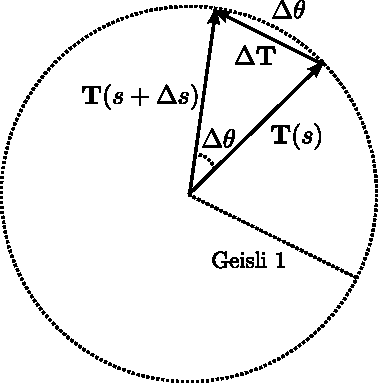
\includegraphics{krappi}} \end {center}
\end {figure}      



\subsection{Hjúfurplan}
 \subsubsection{Skilgreining 3.\arabic{mycount}}\stepcounter{mycount}
   Látum $\cal C$ vera feril í plani eða rúmi og $\rv$ stikun á $\cal C$ með bogalengd.  

{\em Hjúfurplanið} (e.~osculating plane) við ferilinn í punkti $\rv(s)$ er planið sem spannað er af  vigrunum $\Tv(s)$ og $\Nv(s)$ og liggur um punktinn $\rv(s)$.

{\em Hjúfurhringur} (e.~osculating circle) við ferilinn í punkti
$\rv(s)$ er hringur sem liggur í hjúfurplaninu, fer í gegnum punktinn
$\rv(s)$, hefur geisla $\rho(s)$ og hefur miðju í punktinum
$\rv(s)+\rho(s)\Nv(s)$. 
 



\subsection{Tvíþverill}
 \subsubsection{Skilgreining 3.\arabic{mycount}}\stepcounter{mycount}
   Látum $\cal C$ vera feril í plani eða rúmi og
$\rv$ stikun á $\cal C$ með bogalengd.  Vigurinn  
$$\Bv(s)=\Tv(s)\times \Nv(s)$$
kallas {\em tvíþverill} (e.~binormal) við ferilinn í $\rv(s)$.
 

 \bigskip
 $\{\Tv(s),\Nv(s),\Bv(s)\}$ er þverstaðlaður grunnur og kallast \textbf{Frenet ramminn}.


\subsection{Vindingur}
 \subsubsection{Setning og skilgreining 3.\arabic{mycount}}\stepcounter{mycount}
  Látum $\cal C$ vera feril í plani
eða rúmi og $\rv$ stikun á $\cal C$ með bogalengd.  Vigurinn $\Bv'(s)$ er
samsíða vigrinum $\Nv(s)$, þ.e.a.s.~$\Bv'(s)$ er margfeldi af $\Nv(s)$.
Talan $\tau(s)$ þannig að  
$$\Bv'(s)=-\tau(s)\Nv(s)$$
kallast {\em vindingur} ferilsins í punktinum $\rv(s)$.

 




\subsection{Frenet-Serret jöfnurnar}
 \subsubsection{Jöfnur 3.\arabic{mycount}}\stepcounter{mycount}
   Látum $\cal C$ vera feril í plani
eða rúmi og $\rv$ stikun á $\cal C$ með bogalengd.  Þá gildir 
\begin{align*}
\Tv'(s)&=\kappa\Nv\\
\Nv'(s)&=-\kappa\Tv+\tau\Bv\\
\Bv'(s)&=-\tau\Nv.
\end{align*}
 



\subsection{}
 \subsubsection{Setning 3.\arabic{mycount}}\stepcounter{mycount}
   Látum $\cal C$ vera feril í plani eða rúmi. 
Gerum ráð fyrir að $\rv$ sé þjáll stikaferill
sem stikar $\cal C$. Ritum $\vv=\rv'(t)$ og $\av=\rv''(t)$.
Þá gildir í punktinum $\rv(t)$ að
$$\Tv=\frac{\vv}{|\vv|},\qquad 
\Bv=\frac{\vv\times\av}{|\vv\times\av|},\qquad
\Nv=\Bv\times\Tv,$$
einnig er 
$$\kappa=\frac{|\vv\times\av|}{|\vv|^3},\qquad\qquad
\tau=\frac{(\vv\times\av)\cdot \frac{d}{dt}\av}{|\vv\times\av|^2}.$$

 



\end{document}
